\documentclass[12pt, a4paper]{article}

\usepackage[utf8]{inputenc}
\usepackage[T1]{fontenc}
\usepackage[spanish]{babel}
\usepackage{amsmath, amssymb}
\usepackage{geometry}
\usepackage{graphicx}
\usepackage{float}
\usepackage{booktabs}
\usepackage{hyperref}
\usepackage{parskip}
\usepackage{lmodern}

\geometry{top=2.5cm, bottom=2.5cm, left=3cm, right=3cm}

\hypersetup{colorlinks=true, linkcolor=blue!60!black}

\title{
    \Large \textbf{Masa unida a resorte no lineal con amortiguamiento viscoso no lineal} \\[0.5cm]
    \large Simulación y comparación con el sistema lineal
}
\author{}
\date{}

\begin{document}

\maketitle
\tableofcontents
\newpage

% ══════════════════════════════════════════════════════════════════════════════
\section{Introducción}

El objetivo de este trabajo es estudiar el comportamiento dinámico de un sistema masa-resorte cuya rigidez y amortiguamiento son no lineales, y compararlo con el caso lineal clásico. El interés está en ver cómo las no linealidades modifican la frecuencia de oscilación, la tasa de decaimiento y la trayectoria en el espacio de fases.

% ══════════════════════════════════════════════════════════════════════════════
\section{Modelo del sistema}

Una masa $m$ oscila verticalmente sujeta a un resorte con rigidez variable y un amortiguador no lineal (Figura~\ref{fig:sistema}). El sistema se describe con dos ecuaciones de primer orden:

\begin{equation}
    \dot{x}(t) = v(t)
\end{equation}

\begin{equation}
    \dot{v}(t) = -\frac{b}{m}\,|v(t)|^{0{,}5}\,v(t)
                 - \frac{k}{m}\,x(t)\bigl(1 + \alpha\,x^2(t)\bigr) - g
    \label{eq:vdot}
\end{equation}

donde $x(t)$ es el desplazamiento respecto al equilibrio (positivo hacia abajo) y $v(t)$ es la velocidad.

\begin{figure}[H]
    \centering
    \fbox{
        \includegraphics[width=0.3\textwidth]{sistema-masa-resorte.png}
    }
    \caption{Sistema masa-resorte no lineal.}
    \label{fig:sistema}
\end{figure}

\subsection{Interpretación de la ecuación de movimiento}

La aceleración $\dot{v}(t)$ resulta de tres efectos que actúan simultáneamente:

\begin{itemize}
    \item \textbf{Amortiguamiento:} el término $-\frac{b}{m}|v|^{0{,}5}v$ frena la masa en proporción a su velocidad. Al ser no lineal, disipa más energía a velocidades altas pero menos que un amortiguador lineal a velocidades bajas, lo que hace que el sistema tarde más en detenerse cerca del equilibrio.

    \item \textbf{Resorte:} el término $-\frac{k}{m}x(1+\alpha x^2)$ restaura la masa hacia el equilibrio. La rigidez efectiva $k(1+\alpha x^2)$ crece con el desplazamiento: el resorte es más rígido cuanto más se estira, lo que aumenta la frecuencia de oscilación para amplitudes grandes.

    \item \textbf{Gravedad:} el término $-g$ desplaza el punto de equilibrio efectivo, de modo que la masa no oscila exactamente alrededor de $x=0$.
\end{itemize}

\subsection{Parámetros y condiciones iniciales}

\begin{table}[H]
    \centering
    \caption{Parámetros del sistema.}
    \begin{tabular}{clcc}
        \toprule
        \textbf{Parámetro} & \textbf{Descripción} & \textbf{Valor} & \textbf{Unidades} \\
        \midrule
        $m$      & Masa                                   & $1$   & kg \\
        $b$      & Coeficiente de amortiguamiento no lineal & $0{,}5$ & N$\cdot$s$^{1{,}5}$/m$^{1{,}5}$ \\
        $k$      & Constante elástica lineal              & $20$  & N/m \\
        $\alpha$ & Coeficiente de no linealidad           & $0{,}1$ & m$^{-2}$ \\
        $g$      & Aceleración gravitatoria               & $9{,}8$ & m/s$^2$ \\
        \bottomrule
    \end{tabular}
\end{table}

Condiciones iniciales: $x(0) = 1$ m, $v(0) = 0$ m/s.

% ══════════════════════════════════════════════════════════════════════════════
\section{Simulación numérica}

Se integra el sistema mediante un método numérico con paso fijo $h = 0{,}001$ s durante un máximo de 50 unidades de tiempo. La simulación se detiene anticipadamente si $|x(t)| < 0{,}001$ y $|v(t)| < 0{,}001$, lo que indica que el sistema alcanzó el reposo.

% ══════════════════════════════════════════════════════════════════════════════
\section{Resultados}

Con el objetivo de comparar los métodos de integración numérica, se simuló el mismo sistema no lineal utilizando los métodos de Euler y Runge-Kutta de cuarto orden (RK4). Los resultados se analizaron tanto en la evolución temporal de las variables como en el espacio de fases.

\subsection{Evolución temporal}

La Figura \ref{fig:evolucion-comparacion} muestra la evolución temporal del desplazamiento y la velocidad obtenida mediante ambos métodos numéricos. Se utilizó el mismo conjunto de parámetros y condiciones iniciales para garantizar una comparación consistente.

\begin{figure}[H]
    \centering
    \fbox{
        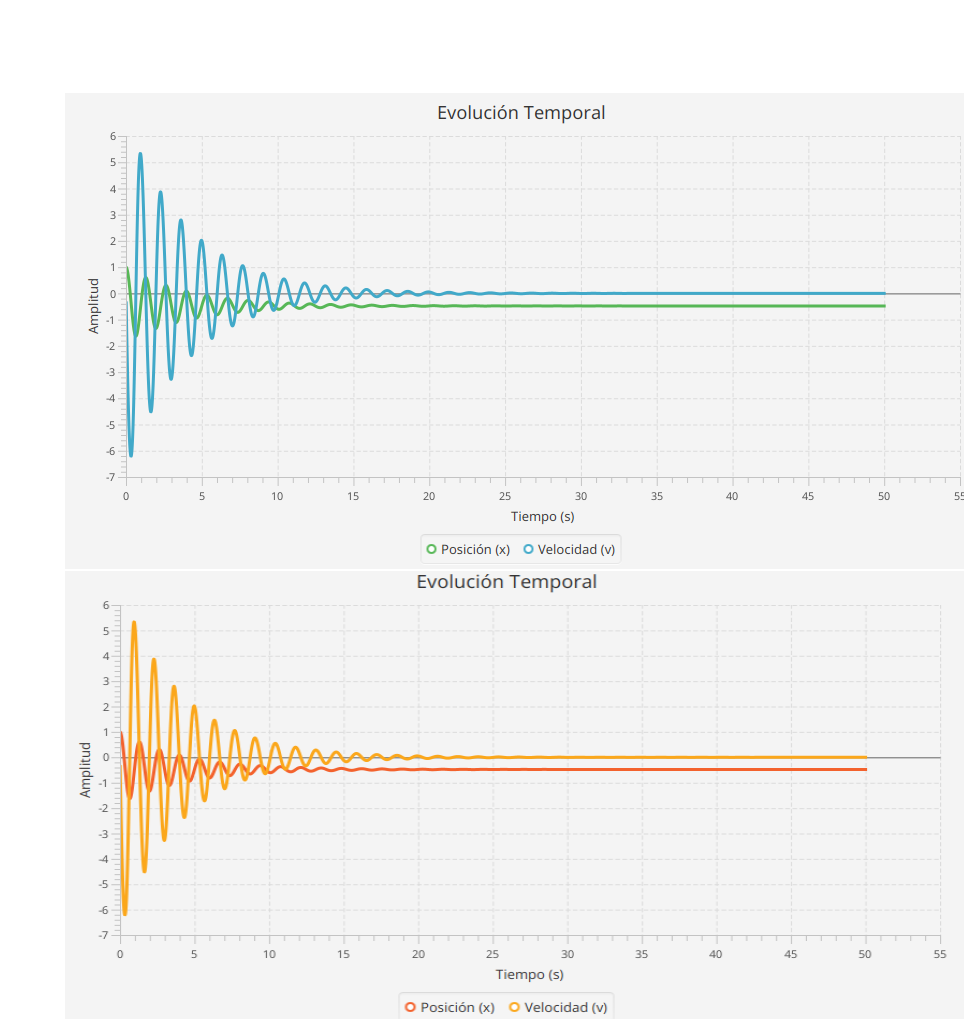
\includegraphics[width=0.8\textwidth]{comparacion-euler-rk4-tiempo.png}
    }
    \caption{Comparación de la evolución temporal del sistema no lineal utilizando los métodos de RK4 y Euler.}
    \label{fig:evolucion-comparacion}
\end{figure}

Puede observarse que ambos métodos reproducen el comportamiento oscilatorio general del sistema. Sin embargo, el método de Euler presenta una mayor acumulación de error numérico a medida que avanza la simulación, mientras que RK4 mantiene una trayectoria más estable y precisa.

\subsection{Diagrama de fase}

La Figura \ref{fig:fase-comparacion} muestra el diagrama de fase obtenido para ambos métodos de integración.

\begin{figure}[H]
    \centering
    \fbox{
        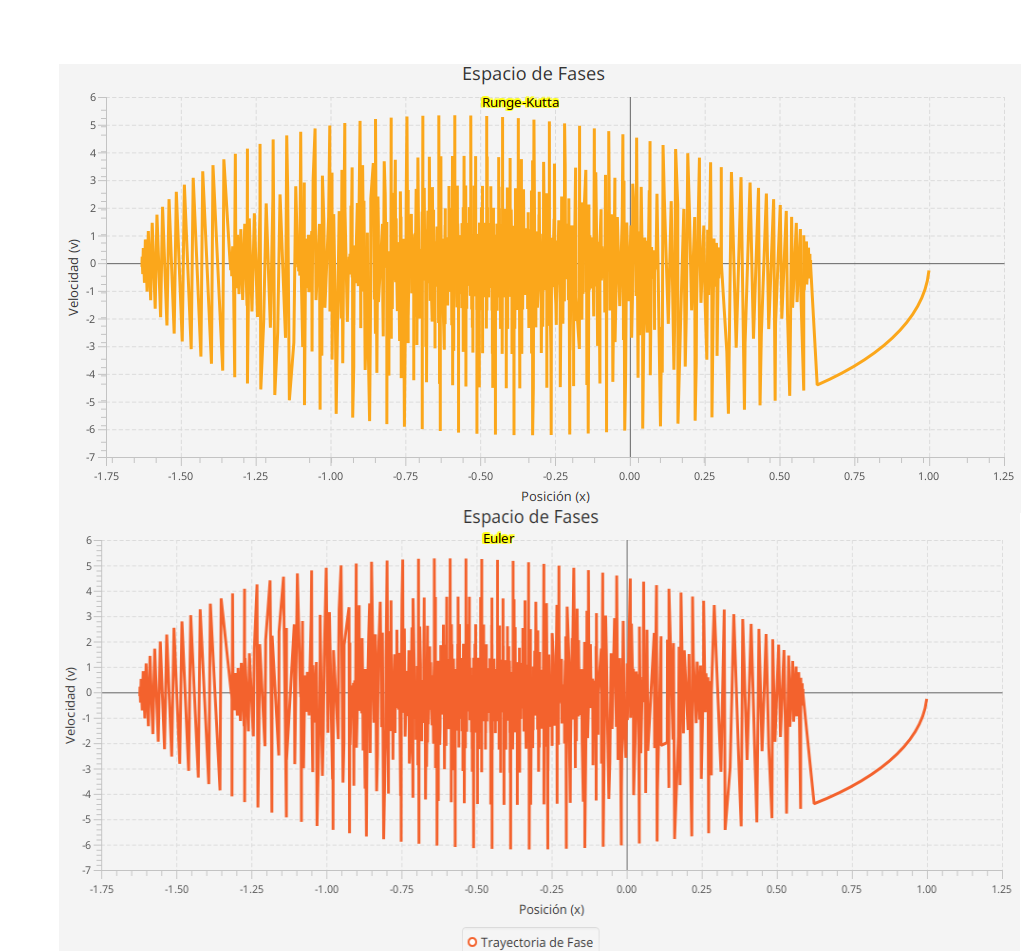
\includegraphics[width=0.8\textwidth]{comparacion-euler-rk4-fase.png}
    }
    \caption{Comparación de los diagramas de fase del sistema no lineal obtenidos mediante RK4 y Euler.}
    \label{fig:fase-comparacion}
\end{figure}

En el espacio de fases se aprecia con mayor claridad el efecto de los errores numéricos. La trayectoria calculada mediante RK4 conserva mejor la forma esperada del movimiento, mientras que el método de Euler muestra desviaciones acumulativas que modifican gradualmente la geometría de la órbita.

\subsection{Comparación de precisión}

El método de Euler es sencillo de implementar y posee un bajo costo computacional, pero su precisión es de primer orden, por lo que los errores crecen rápidamente cuando se utilizan pasos de integración relativamente grandes. Por otro lado, RK4 presenta precisión de cuarto orden y produce resultados considerablemente más cercanos a la solución real del sistema.

Para el sistema no lineal analizado, RK4 logró mantener la estabilidad numérica durante toda la simulación y representar con mayor fidelidad la dinámica del oscilador. En consecuencia, resulta el método más adecuado cuando se requiere precisión en simulaciones de larga duración o en sistemas con comportamiento complejo.

% ══════════════════════════════════════════════════════════════════════════════
\section{Comparación: sistema lineal vs.\ no lineal}

A partir de las simulaciones realizadas puede observarse que ambos sistemas presentan un comportamiento cualitativamente similar. En los dos casos la masa realiza oscilaciones amortiguadas alrededor de una posición de equilibrio desplazada respecto del origen debido a la acción de la gravedad. La amplitud de las oscilaciones disminuye progresivamente con el tiempo hasta que el sistema alcanza el estado estacionario.

En las gráficas de evolución temporal se observa que tanto el sistema lineal como el no lineal parten de las mismas condiciones iniciales y convergen hacia una posición de equilibrio cercana a $x \approx -0{,}5$ m. Esta posición coincide con el punto donde las fuerzas elásticas y gravitatorias se equilibran. La velocidad también converge a cero en ambos casos, indicando que la energía mecánica del sistema se disipa por efecto del amortiguamiento.

\begin{figure}[H]
    \centering
    \fbox{
        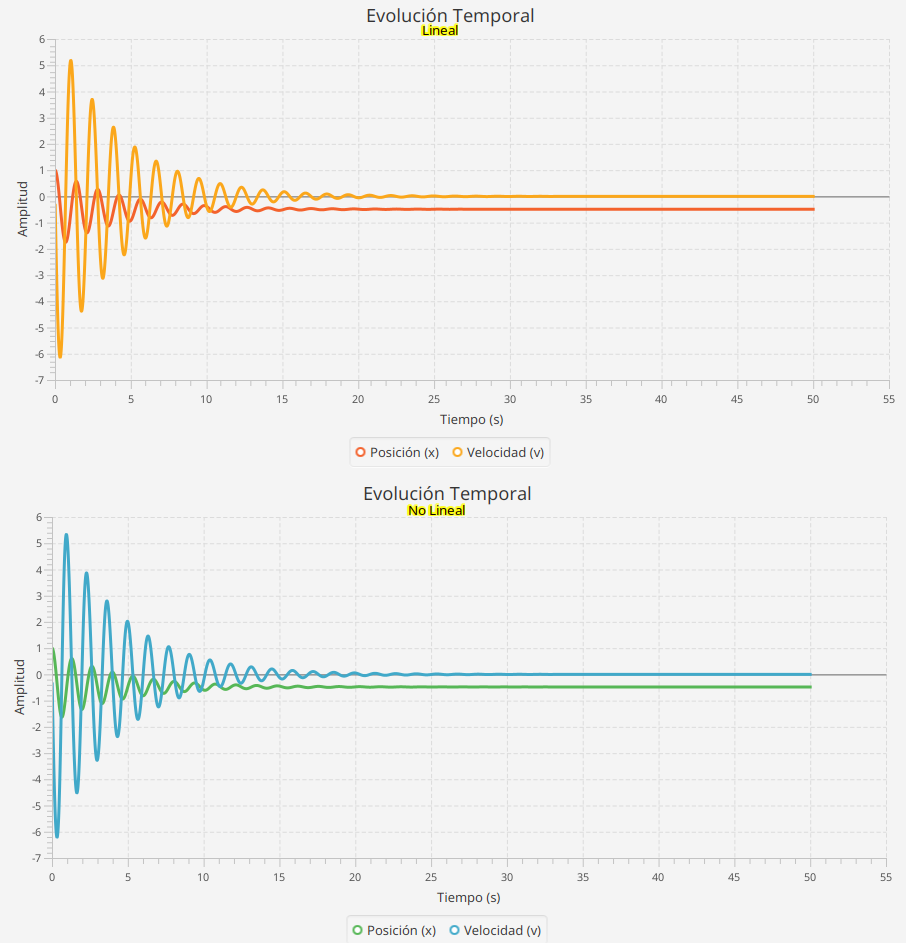
\includegraphics[width=0.8\textwidth]{comparacion-lineal-no-lineal-tiempo.png}
    }
    \caption{Comparación de la evolución temporal del sistmea Lineal y No Lineal}
    \label{fig:evolucion-comparacion}
\end{figure}

Las diferencias entre ambos modelos son más evidentes durante las primeras oscilaciones, cuando los desplazamientos y velocidades alcanzan valores elevados. En el sistema no lineal, la fuerza restauradora está dada por

[
F_r = -k,x(1+\alpha x^2),
]

por lo que la rigidez efectiva aumenta con la amplitud de la oscilación. Esto provoca ligeras variaciones en la frecuencia respecto del sistema lineal, cuya constante elástica permanece fija durante toda la evolución.

Asimismo, el término de amortiguamiento no lineal

[
F_a = -b,|v|^{0.5}v
]

produce una disipación de energía dependiente del estado del sistema. Como consecuencia, la reducción de amplitud no sigue exactamente el mismo patrón que en el caso lineal. Sin embargo, dado que el coeficiente de no linealidad utilizado es relativamente pequeño ($\alpha = 0{,}1$), las diferencias observadas son moderadas y ambos sistemas mantienen una respuesta dinámica muy similar.

Los diagramas de fase permiten visualizar con mayor claridad estas características. En ambos casos se obtiene una espiral convergente hacia el punto de equilibrio, lo que confirma que los sistemas son estables. El sistema lineal presenta una espiral prácticamente elíptica y uniforme, característica de un oscilador armónico amortiguado. Por otro lado, el sistema no lineal exhibe una trayectoria ligeramente deformada, especialmente en las órbitas externas correspondientes a las oscilaciones de mayor amplitud. Estas deformaciones son consecuencia directa de la dependencia no lineal de la rigidez y del amortiguamiento.

\begin{figure}[H]
    \centering
    \fbox{
        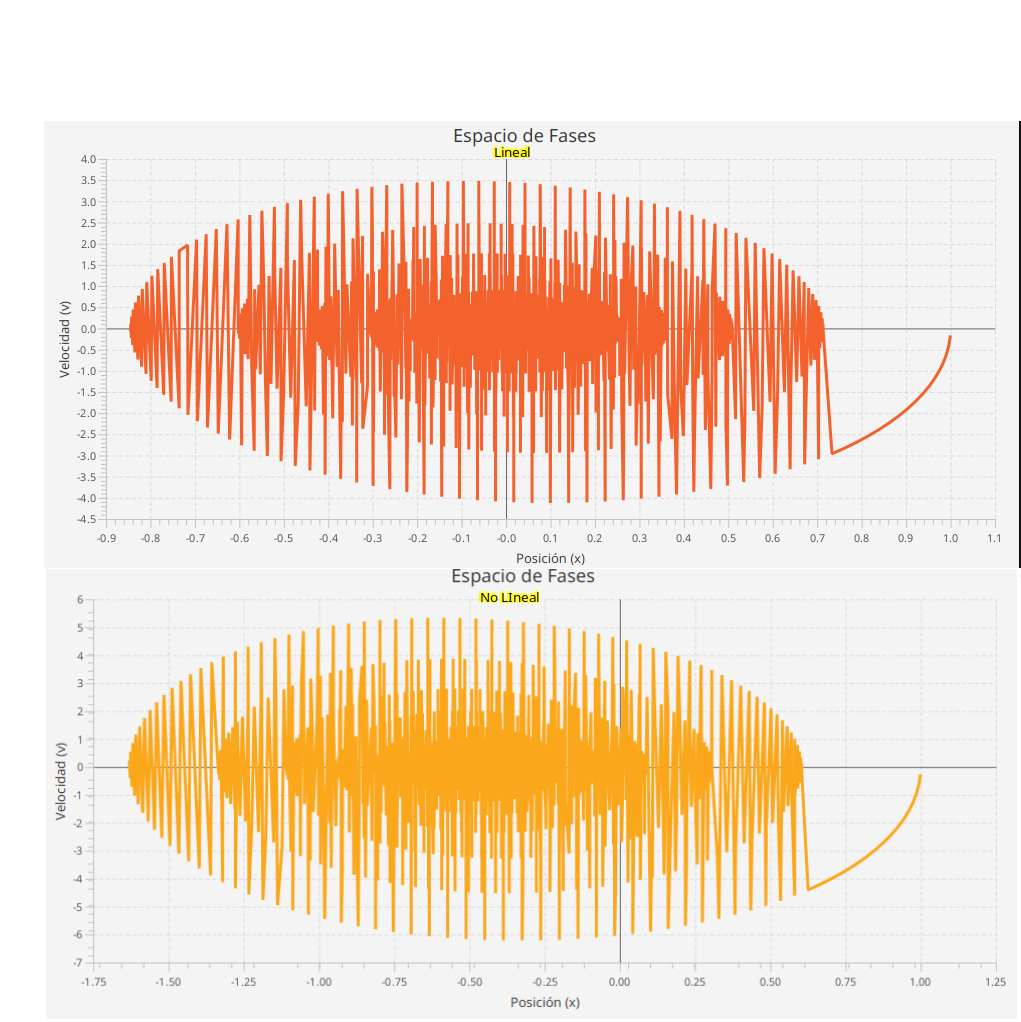
\includegraphics[width=0.7\textwidth]{comparacion-lineal-no-lineal-fase.png}
    }
    \caption{Comparación de los diagramas de fase del sistema Lineal y No Lineal}
    \label{fig:fase-comparacion}
\end{figure}

A medida que la amplitud disminuye, las trayectorias de ambos sistemas se vuelven cada vez más parecidas. Esto ocurre porque, cerca del equilibrio, los términos no lineales tienen una influencia mucho menor y la dinámica del sistema se aproxima a la de un oscilador lineal amortiguado.

% ══════════════════════════════════════════════════════════════════════════════
% ══════════════════════════════════════════════════════════════════════════════
\section{Análisis con cambio de datos iniciales}

Para estudiar la influencia de la no linealidad en el comportamiento dinámico del sistema, se modificó el coeficiente de no linealidad \(\alpha\), asignándole un valor de \(\alpha = 1.0\). Este parámetro multiplica el término no lineal de la fuerza restauradora y permite evaluar cómo se altera la dinámica respecto del caso lineal.

La Figura \ref{fig:no-linealidad} presenta los resultados obtenidos para la evolución temporal y el espacio de fases utilizando el método de Runge-Kutta de cuarto orden (RK4).

\begin{figure}[H]
    \centering
    \fbox{
        \includegraphics[width=0.9\textwidth]{rk4-evol-fases-no-linealidad-1.png}
    }
    \caption{Evolución temporal y espacio de fases para \(\alpha = 1.0\).}
    \label{fig:no-linealidad}
\end{figure}

En la evolución temporal se observa que tanto la posición como la velocidad presentan oscilaciones amortiguadas cuya amplitud disminuye progresivamente hasta alcanzar el estado de equilibrio. Este comportamiento indica que el término disipativo continúa siendo dominante en escalas temporales largas, provocando la pérdida gradual de energía del sistema.

Por otra parte, el espacio de fases revela con mayor claridad el efecto de la no linealidad. A diferencia de un oscilador lineal ideal, donde las trayectorias poseen formas regulares y predecibles, la incorporación del término no lineal modifica la relación entre posición y velocidad, produciendo trayectorias más complejas. Esto evidencia que la fuerza restauradora ya no es proporcional únicamente al desplazamiento, sino que depende de términos de orden superior.

La comparación con el caso lineal permite concluir que el parámetro \(\alpha\) influye directamente en la dinámica del sistema. Para \(\alpha = 1.0\) los efectos no lineales ya son apreciables, especialmente en el espacio de fases, aunque el sistema conserva el carácter oscilatorio amortiguado general. Esto demuestra que pequeñas variaciones en el coeficiente de no linealidad pueden modificar la evolución de las trayectorias y alterar la respuesta dinámica del sistema.

% ══════════════════════════════════════════════════════════════════════════════
\section{Conclusiones}

Se simuló un sistema masa-resorte no lineal mediante los métodos de Euler y RK4, analizando su evolución temporal y espacio de fases. La comparación demostró que, aunque ambos métodos capturan la dinámica oscilatoria, RK4 ofrece mayor estabilidad y precisión, siendo el método más adecuado para este estudio.Los resultados confirmaron la estabilidad del sistema y cómo el amortiguamiento disipa la energía hasta el equilibrio. Asimismo, se observó que al aumentar el coeficiente de no linealidad ($\alpha$), el comportamiento se aleja del modelo lineal, generando trayectorias complejas y deformaciones en el espacio de fases. En definitiva, este trabajo resalta la necesidad de elegir métodos de integración robustos y subraya cómo los términos no lineales permiten capturar fenómenos físicos que los modelos lineales clásicos omiten.


\end{document}